%-*-latex-*-
\sectionthree{Build heap}
\begin{python0}
from solutions import *; clear()
\end{python0}

Frequently, you want to make an array into a heap.
This is called
\defterm{build-maxheap}\tinysidebar{build-maxheap \\ build-minheap \\ build-heap \\ max-heapify \\ min-heapify \\ heapify}
(if you want to make
the array into a maxheap)
or otherwise it's called
\defterm{build-minheap}.
I'll just call it \defterm{build-heap}
if the type of heap is clear from the context.
It's also called
\defterm{max-heapify}
or
\defterm{min-heapify}
or
\defterm{heapify} (if the context is clear).


\subsection{Slow method}

We can use the heaps to sort arrays.
For instance suppose you have an array
\verb!x! of 10 values.
Looking just at the first value, \verb!x[0]!,
you have a heap of one
value.
Now insert \verb!x[1]! into the heap with only
\verb!x[0]!.
At this point \verb!x[0..1]! is a heap --
say we want to sort it in 
ascending order, which means that we're using maxheap
(you see why later).
Now we repeat to get \verb!x[0..2]! to be a maxheap.
Etc.
When we're done, we have a maxheap of \verb!x[0..9]!.
Inserting into a heap requires $\log_2 n$ steps
where $n$ is the
size of the heap.
Therefore the 
runtime to create the heap 
from an array of $n$ values is, informally speaking, 
$\log_2 1 + \log_2 2 + \cdots + \log_2 n$
which is $\log_2 n! \leq \log_2 n^n = n \log_2 n$.
There's a faster algorithm ... the real build-heap.




\subsection{Fast and right method}

Now for the real build-heap or build-maxheap or build-minheap.

As mentioned at the beginning of this section,
you can create the maxheap by continually inserting values into the
the maxheap.
The runtime is $O(n \log n)$.
Instead of doing that you can
also execute heapify-down on all the non-leaves positions
of the given array is a systematic way: from the non-leaf at the
lowest level to the root, more or less the opposite of the
breadth-first traversal (ignoring the leaves).

Note that if the size of the array is $n$,
then the indices of the leaves are
$n/2$ (integer division), $n/2 + 1$, ..., $n - 1$.
Therefore you can convert the array to a maxheap
if you perform heapify-down at indices
$n/2, n/2-1, n/2-2,...,0$, you will get a maxheap too.

The runtime of build-heap is
\[
  \lg (n/2) + \lg (n/2 + 1) + \cdots + \lg n
\]
Each of these terms are $\leq \lg n$ and there are $n/2$
such heapify operations.
So the runtime is at most $(n/2) \lg n = O(n \lg n)$.
But that's an over-approximation.
It can be shown that the runtime is actually
\[
O(n)
\]
which is faster than the earlier build max heap algorithm
at the beginning of this section.
However this does not improve the overall heapsort
since the second part of the heapsort process will still run
in $O(n \log n)$.

\begin{console}
ALGORITHM: build_maxheap (or heapify)
INPUT: x - array containing n values x[0..n-1] that will
           represent a maxheap at the end of this
           algorithm.
       n - length of x

Perform heapify bottom-up from the first nonleaf to the
root, i.e.,

for i = n/2, n/2 - 1, n/2 - 2, ..., 0:
    perform heapify-down on x at i
\end{console}

As mentioned at the beginning of this section, the runtime of
this build-maxheap has runtime
\[
O(n)
\]

Let me show you how to 
build a maxheap given an array.
Let's say we're given this array:
\[
1, 0, 9, 8, 3, 2, 4, 7, 6
\]
Here's the array drawn as a complete tree:

\begin{center}
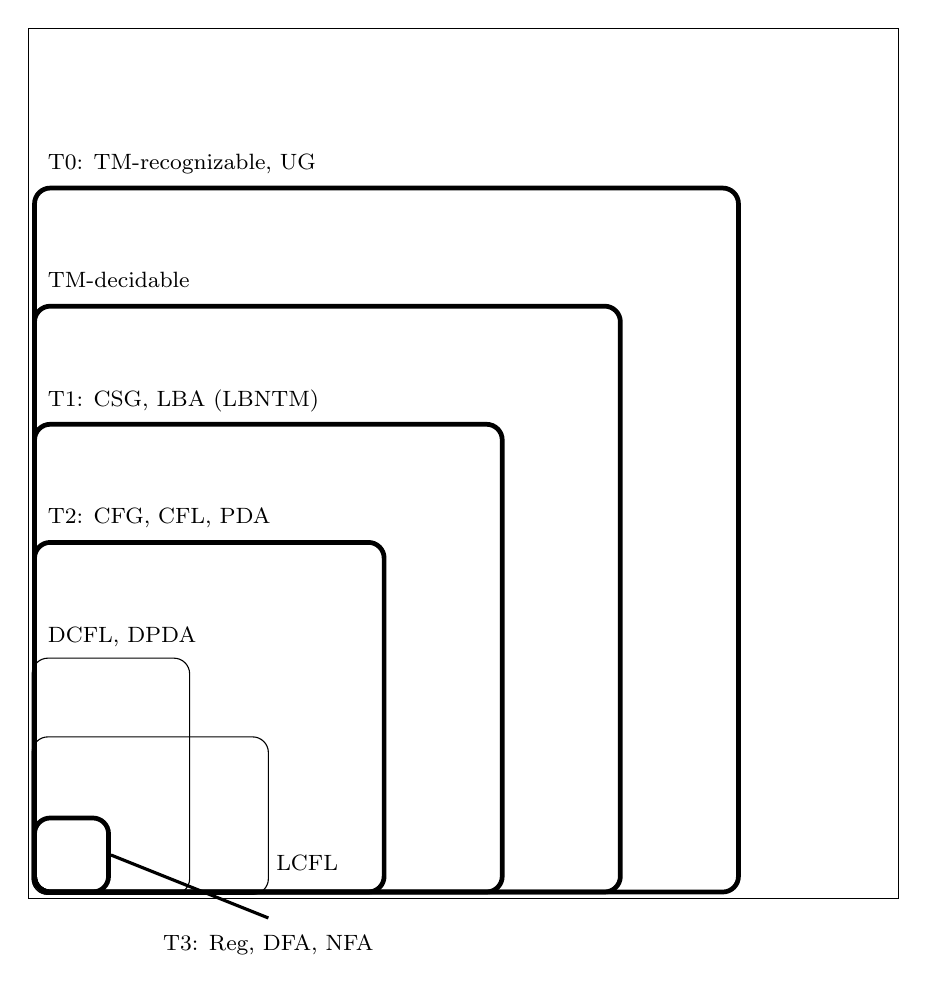
\begin{tikzpicture}

\draw (5.475, 5.475)
  node[draw, , , color=black,
       rounded corners=0cm, inner sep=0cm] {

\begin{minipage}[t][11.05cm]{11.05cm}
\mbox{}

\end{minipage}

};
\draw (0.5, 0.5)
  node[draw, line width=0.06cm, , color=black,
       rounded corners=0.2cm, inner sep=0cm] {

\begin{minipage}[t][0.94cm]{0.94cm}
\mbox{}

\end{minipage}

};
\draw (3.0, -0.65)
  node[draw=none, line width=0cm, , color=black,
       rounded corners=0cm, inner sep=0cm] {

\begin{minipage}[t][0.7cm]{2cm}
\mbox{}

\end{minipage}

};\draw (3.0, -0.65) node[color=black] {{\footnotesize T3: Reg, DFA, NFA}};\draw[line width=0.04cm,black] (1,0.5) to  (3.0,-0.3);

\draw (1.0, 1.5)
  node[draw, , , color=black,
       rounded corners=0.2cm, inner sep=0cm] {

\begin{minipage}[t][3.0cm]{2.0cm}
\mbox{}

\end{minipage}

};
\draw (2.6, 3.3)
  node[draw=none, line width=0cm, , color=black,
       rounded corners=0cm, inner sep=0cm] {

\begin{minipage}[t][0.1cm]{4.8cm}
\mbox{}

\end{minipage}

};
\draw (2.6, 3.3) node[color=black,
 inner sep=0cm] {
 
\begin{minipage}[t][0.1cm]{4.8cm}
{\footnotesize DCFL, DPDA}
\end{minipage}

};
\draw (1.5, 1.0)
  node[draw, , , color=black,
       rounded corners=0.2cm, inner sep=0cm] {

\begin{minipage}[t][2.0cm]{3.0cm}
\mbox{}

\end{minipage}

};
\draw (4.1, 0.4)
  node[draw=none, line width=0cm, , color=black,
       rounded corners=0cm, inner sep=0cm] {

\begin{minipage}[t][0.1cm]{2.0cm}
\mbox{}

\end{minipage}

};
\draw (4.1, 0.4) node[color=black,
 inner sep=0cm] {
 
\begin{minipage}[t][0.1cm]{2.0cm}
{\footnotesize LCFL}
\end{minipage}

};
\draw (2.25, 2.25)
  node[draw, line width=0.06cm, , color=black,
       rounded corners=0.2cm, inner sep=0cm] {

\begin{minipage}[t][4.44cm]{4.44cm}
\mbox{}

\end{minipage}

};
\draw (2.85, 4.8)
  node[draw=none, line width=0cm, , color=black,
       rounded corners=0cm, inner sep=0cm] {

\begin{minipage}[t][0.1cm]{5.3cm}
\mbox{}

\end{minipage}

};
\draw (2.85, 4.8) node[color=black,
 inner sep=0cm] {
 
\begin{minipage}[t][0.1cm]{5.3cm}
{\footnotesize T2: CFG, CFL, PDA}
\end{minipage}

};
\draw (3.0, 3.0)
  node[draw, line width=0.06cm, , color=black,
       rounded corners=0.2cm, inner sep=0cm] {

\begin{minipage}[t][5.94cm]{5.94cm}
\mbox{}

\end{minipage}

};
\draw (2.85, 6.3)
  node[draw=none, line width=0cm, , color=black,
       rounded corners=0cm, inner sep=0cm] {

\begin{minipage}[t][0.1cm]{5.3cm}
\mbox{}

\end{minipage}

};
\draw (2.85, 6.3) node[color=black,
 inner sep=0cm] {
 
\begin{minipage}[t][0.1cm]{5.3cm}
{\footnotesize T1: CSG, LBA (LBNTM)}
\end{minipage}

};
\draw (3.75, 3.75)
  node[draw, line width=0.06cm, , color=black,
       rounded corners=0.2cm, inner sep=0cm] {

\begin{minipage}[t][7.44cm]{7.44cm}
\mbox{}

\end{minipage}

};
\draw (2.85, 7.8)
  node[draw=none, line width=0cm, , color=black,
       rounded corners=0cm, inner sep=0cm] {

\begin{minipage}[t][0.1cm]{5.3cm}
\mbox{}

\end{minipage}

};
\draw (2.85, 7.8) node[color=black,
 inner sep=0cm] {
 
\begin{minipage}[t][0.1cm]{5.3cm}
{\footnotesize TM-decidable}
\end{minipage}

};
\draw (4.5, 4.5)
  node[draw, line width=0.06cm, , color=black,
       rounded corners=0.2cm, inner sep=0cm] {

\begin{minipage}[t][8.94cm]{8.94cm}
\mbox{}

\end{minipage}

};
\draw (2.85, 9.3)
  node[draw=none, line width=0cm, , color=black,
       rounded corners=0cm, inner sep=0cm] {

\begin{minipage}[t][0.1cm]{5.3cm}
\mbox{}

\end{minipage}

};
\draw (2.85, 9.3) node[color=black,
 inner sep=0cm] {
 
\begin{minipage}[t][0.1cm]{5.3cm}
{\footnotesize T0: TM-recognizable, UG}
\end{minipage}

};
\end{tikzpicture}

\end{center}



The main idea of build-maxheap
is to maintain a collection of subheaps.
Each leaf is already a heap.
So I actually start with 5 subheaps:

\begin{center}
\begin{tikzpicture}

\fill[blue!10] (0.0, 0.0) circle (0.35);
\node [line width=0.03cm,black,minimum size=0.6699999999999999cm,draw,circle] at (0.0,0.0)(1){};\draw (0.0, 0.0) node[color=black] {\texttt{1}};
\fill[blue!10] (-1.9, -1.0) circle (0.35);
\node [line width=0.03cm,black,minimum size=0.6699999999999999cm,draw,circle] at (-1.9,-1.0)(0){};\draw (-1.9, -1.0) node[color=black] {\texttt{0}};
\fill[blue!10] (1.9, -1.0) circle (0.35);
\node [line width=0.03cm,black,minimum size=0.6699999999999999cm,draw,circle] at (1.9,-1.0)(9){};\draw (1.9, -1.0) node[color=black] {\texttt{9}};
\fill[blue!10] (-2.85, -2.0) circle (0.35);
\node [line width=0.03cm,black,minimum size=0.6699999999999999cm,draw,circle] at (-2.85,-2.0)(8){};\draw (-2.85, -2.0) node[color=black] {\texttt{8}};
\fill[blue!10] (-0.95, -2.0) circle (0.35);
\node [line width=0.03cm,black,minimum size=0.6699999999999999cm,draw,circle] at (-0.95,-2.0)(3){};\draw (-0.95, -2.0) node[color=black] {\texttt{3}};
\fill[blue!10] (0.95, -2.0) circle (0.35);
\node [line width=0.03cm,black,minimum size=0.6699999999999999cm,draw,circle] at (0.95,-2.0)(2){};\draw (0.95, -2.0) node[color=black] {\texttt{2}};
\fill[blue!10] (2.85, -2.0) circle (0.35);
\node [line width=0.03cm,black,minimum size=0.6699999999999999cm,draw,circle] at (2.85,-2.0)(4){};\draw (2.85, -2.0) node[color=black] {\texttt{4}};
\fill[blue!10] (-3.33, -3.0) circle (0.35);
\node [line width=0.03cm,black,minimum size=0.6699999999999999cm,draw,circle] at (-3.33,-3.0)(7){};\draw (-3.33, -3.0) node[color=black] {\texttt{7}};
\fill[blue!10] (-2.38, -3.0) circle (0.35);
\node [line width=0.03cm,black,minimum size=0.6699999999999999cm,draw,circle] at (-2.38,-3.0)(6){};\draw (-2.38, -3.0) node[color=black] {\texttt{6}};\draw[line width=0.03cm,black] (1) to  (0);
\draw[line width=0.03cm,black] (1) to  (9);
\draw[line width=0.03cm,black] (0) to  (8);
\draw[line width=0.03cm,black] (0) to  (3);
\draw[line width=0.03cm,black] (9) to  (2);
\draw[line width=0.03cm,black] (9) to  (4);
\draw[line width=0.03cm,black] (8) to  (7);
\draw[line width=0.03cm,black] (8) to  (6);
\node [ellipse, draw=red, fit=(3), line width=0.1cm, inner sep=0.0cm] {};\node [ellipse, draw=red, fit=(2), line width=0.1cm, inner sep=0.0cm] {};\node [ellipse, draw=red, fit=(4), line width=0.1cm, inner sep=0.0cm] {};\node [ellipse, draw=red, fit=(7), line width=0.1cm, inner sep=0.0cm] {};\node [ellipse, draw=red, fit=(6), line width=0.1cm, inner sep=0.0cm] {};
\end{tikzpicture}

\end{center}



I now heapify in this order: 8,9,0,1.
By this I mean \verb!8! (at index 3) is going to start off at the
root postion of the heap that combines two subheaps at 7 and 6.


\textsc{Step 1.}
I heapify-down at \texttt{8} (at index 3).
There's no change since the
subtree at \texttt{8} is a maxheap.

\begin{center}
\begin{tikzpicture}

\fill[blue!10] (0.0, 0.0) circle (0.35);
\node [line width=0.03cm,black,minimum size=0.6699999999999999cm,draw,circle] at (0.0,0.0)(1){};\draw (0.0, 0.0) node[color=black] {\texttt{1}};
\fill[blue!10] (-1.9, -1.0) circle (0.35);
\node [line width=0.03cm,black,minimum size=0.6699999999999999cm,draw,circle] at (-1.9,-1.0)(0){};\draw (-1.9, -1.0) node[color=black] {\texttt{0}};
\fill[blue!10] (1.9, -1.0) circle (0.35);
\node [line width=0.03cm,black,minimum size=0.6699999999999999cm,draw,circle] at (1.9,-1.0)(9){};\draw (1.9, -1.0) node[color=black] {\texttt{9}};
\fill[blue!10] (-2.85, -2.0) circle (0.35);
\node [line width=0.03cm,black,minimum size=0.6699999999999999cm,draw,circle] at (-2.85,-2.0)(8){};\draw (-2.85, -2.0) node[color=black] {\texttt{8}};
\fill[blue!10] (-0.95, -2.0) circle (0.35);
\node [line width=0.03cm,black,minimum size=0.6699999999999999cm,draw,circle] at (-0.95,-2.0)(3){};\draw (-0.95, -2.0) node[color=black] {\texttt{3}};
\fill[blue!10] (0.95, -2.0) circle (0.35);
\node [line width=0.03cm,black,minimum size=0.6699999999999999cm,draw,circle] at (0.95,-2.0)(2){};\draw (0.95, -2.0) node[color=black] {\texttt{2}};
\fill[blue!10] (2.85, -2.0) circle (0.35);
\node [line width=0.03cm,black,minimum size=0.6699999999999999cm,draw,circle] at (2.85,-2.0)(4){};\draw (2.85, -2.0) node[color=black] {\texttt{4}};
\fill[blue!10] (-3.33, -3.0) circle (0.35);
\node [line width=0.03cm,black,minimum size=0.6699999999999999cm,draw,circle] at (-3.33,-3.0)(7){};\draw (-3.33, -3.0) node[color=black] {\texttt{7}};
\fill[blue!10] (-2.38, -3.0) circle (0.35);
\node [line width=0.03cm,black,minimum size=0.6699999999999999cm,draw,circle] at (-2.38,-3.0)(6){};\draw (-2.38, -3.0) node[color=black] {\texttt{6}};\draw[line width=0.03cm,black] (1) to  (0);
\draw[line width=0.03cm,black] (1) to  (9);
\draw[line width=0.03cm,black] (0) to  (8);
\draw[line width=0.03cm,black] (0) to  (3);
\draw[line width=0.03cm,black] (9) to  (2);
\draw[line width=0.03cm,black] (9) to  (4);
\draw[line width=0.03cm,black] (8) to  (7);
\draw[line width=0.03cm,black] (8) to  (6);
\node [ellipse, draw=red, fit=(3), line width=0.1cm, inner sep=0.0cm] {};\node [ellipse, draw=red, fit=(2), line width=0.1cm, inner sep=0.0cm] {};\node [ellipse, draw=red, fit=(4), line width=0.1cm, inner sep=0.0cm] {};\node [ellipse, draw=red, fit=(8) (7) (6), line width=0.1cm, inner sep=0.0cm] {};
\end{tikzpicture}

\end{center}




\textsc{Step 2.}
Heapify-down at index 2 with value \texttt{9}:
No change since the subtree at \texttt{9} is a maxheap.

\begin{center}
\begin{tikzpicture}

\fill[blue!10] (0.0, 0.0) circle (0.35);
\node [line width=0.03cm,black,minimum size=0.6699999999999999cm,draw,circle] at (0.0,0.0)(1){};\draw (0.0, 0.0) node[color=black] {\texttt{1}};
\fill[blue!10] (-1.9, -1.0) circle (0.35);
\node [line width=0.03cm,black,minimum size=0.6699999999999999cm,draw,circle] at (-1.9,-1.0)(0){};\draw (-1.9, -1.0) node[color=black] {\texttt{0}};
\fill[blue!10] (1.9, -1.0) circle (0.35);
\node [line width=0.03cm,black,minimum size=0.6699999999999999cm,draw,circle] at (1.9,-1.0)(9){};\draw (1.9, -1.0) node[color=black] {\texttt{9}};
\fill[blue!10] (-2.85, -2.0) circle (0.35);
\node [line width=0.03cm,black,minimum size=0.6699999999999999cm,draw,circle] at (-2.85,-2.0)(8){};\draw (-2.85, -2.0) node[color=black] {\texttt{8}};
\fill[blue!10] (-0.95, -2.0) circle (0.35);
\node [line width=0.03cm,black,minimum size=0.6699999999999999cm,draw,circle] at (-0.95,-2.0)(3){};\draw (-0.95, -2.0) node[color=black] {\texttt{3}};
\fill[blue!10] (0.95, -2.0) circle (0.35);
\node [line width=0.03cm,black,minimum size=0.6699999999999999cm,draw,circle] at (0.95,-2.0)(2){};\draw (0.95, -2.0) node[color=black] {\texttt{2}};
\fill[blue!10] (2.85, -2.0) circle (0.35);
\node [line width=0.03cm,black,minimum size=0.6699999999999999cm,draw,circle] at (2.85,-2.0)(4){};\draw (2.85, -2.0) node[color=black] {\texttt{4}};
\fill[blue!10] (-3.33, -3.0) circle (0.35);
\node [line width=0.03cm,black,minimum size=0.6699999999999999cm,draw,circle] at (-3.33,-3.0)(7){};\draw (-3.33, -3.0) node[color=black] {\texttt{7}};
\fill[blue!10] (-2.38, -3.0) circle (0.35);
\node [line width=0.03cm,black,minimum size=0.6699999999999999cm,draw,circle] at (-2.38,-3.0)(6){};\draw (-2.38, -3.0) node[color=black] {\texttt{6}};\draw[line width=0.03cm,black] (1) to  (0);
\draw[line width=0.03cm,black] (1) to  (9);
\draw[line width=0.03cm,black] (0) to  (8);
\draw[line width=0.03cm,black] (0) to  (3);
\draw[line width=0.03cm,black] (9) to  (2);
\draw[line width=0.03cm,black] (9) to  (4);
\draw[line width=0.03cm,black] (8) to  (7);
\draw[line width=0.03cm,black] (8) to  (6);
\node [ellipse, draw=red, fit=(3), line width=0.1cm, inner sep=0.0cm] {};\node [ellipse, draw=red, fit=(9) (2) (4), line width=0.1cm, inner sep=0.0cm] {};\node [ellipse, draw=red, fit=(8) (7) (6), line width=0.1cm, inner sep=0.0cm] {};
\end{tikzpicture}

\end{center}




\textsc{Step 3.}
Heapify-down at index 1 with value \texttt{0}:
I need 2 swaps.
After that the subtree at position where \texttt{0} originally 
was a maxheap.


\begin{center}

\begin{tikzpicture}
\node at (5,-0.8) [minimum size=8mm] (Z) {$$};
\node at (3,-1.6) [circle,draw,minimum size=8mm] (B) {$\alpha$};
\node at (1,-2.4000000000000004) [circle,draw,minimum size=8mm] (A) {$\beta$};
\node at (5,-2.4000000000000004)
    [isosceles triangle, shape border rotate=+90,
     draw,minimum size=8mm,minimum height=2cm,
     anchor=north] (Etriangle) {$T_3$};
\coordinate (E) at (5,-2.4000000000000004);
\node at (0,-3.2)
    [isosceles triangle, shape border rotate=+90,
     draw,minimum size=8mm,minimum height=2cm,
     anchor=north] (Ctriangle) {$T_1$};
\coordinate (C) at (0,-3.2);
\node at (2,-3.2)
    [isosceles triangle, shape border rotate=+90,
     draw,minimum size=8mm,minimum height=2cm,
     anchor=north] (Dtriangle) {$T_2$};
\coordinate (D) at (2,-3.2);
\draw [-,thick] (Z) -- (B);
\draw [-,thick] (B) -- (A);
\draw [-,thick] (A) -- (D);
\draw [-,thick] (A) -- (C);
\draw [-,thick] (B) -- (E);

;
\end{tikzpicture}
    
\end{center}


\textsc{Step 4.}
Heapify-down at index 0 with value \texttt{1}:
I need 2 swaps.
After that the subtree at the place
where \texttt{1} was is a maxheap.

\begin{center}
\begin{tikzpicture}

\fill[blue!10] (0.0, 0.0) circle (0.35);
\node [line width=0.03cm,black,minimum size=0.6699999999999999cm,draw,circle] at (0.0,0.0)(9){};\draw (0.0, 0.0) node[color=black] {\texttt{9}};
\fill[blue!10] (-1.9, -1.0) circle (0.35);
\node [line width=0.03cm,black,minimum size=0.6699999999999999cm,draw,circle] at (-1.9,-1.0)(8){};\draw (-1.9, -1.0) node[color=black] {\texttt{8}};
\fill[blue!10] (1.9, -1.0) circle (0.35);
\node [line width=0.03cm,black,minimum size=0.6699999999999999cm,draw,circle] at (1.9,-1.0)(4){};\draw (1.9, -1.0) node[color=black] {\texttt{4}};
\fill[blue!10] (-2.85, -2.0) circle (0.35);
\node [line width=0.03cm,black,minimum size=0.6699999999999999cm,draw,circle] at (-2.85,-2.0)(7){};\draw (-2.85, -2.0) node[color=black] {\texttt{7}};
\fill[blue!10] (-0.95, -2.0) circle (0.35);
\node [line width=0.03cm,black,minimum size=0.6699999999999999cm,draw,circle] at (-0.95,-2.0)(3){};\draw (-0.95, -2.0) node[color=black] {\texttt{3}};
\fill[blue!10] (0.95, -2.0) circle (0.35);
\node [line width=0.03cm,black,minimum size=0.6699999999999999cm,draw,circle] at (0.95,-2.0)(2){};\draw (0.95, -2.0) node[color=black] {\texttt{2}};
\fill[blue!10] (2.85, -2.0) circle (0.35);
\node [line width=0.03cm,black,minimum size=0.6699999999999999cm,draw,circle] at (2.85,-2.0)(1){};\draw (2.85, -2.0) node[color=black] {\texttt{1}};
\fill[blue!10] (-3.33, -3.0) circle (0.35);
\node [line width=0.03cm,black,minimum size=0.6699999999999999cm,draw,circle] at (-3.33,-3.0)(0){};\draw (-3.33, -3.0) node[color=black] {\texttt{0}};
\fill[blue!10] (-2.38, -3.0) circle (0.35);
\node [line width=0.03cm,black,minimum size=0.6699999999999999cm,draw,circle] at (-2.38,-3.0)(6){};\draw (-2.38, -3.0) node[color=black] {\texttt{6}};\draw[line width=0.03cm,black] (9) to  (8);
\draw[line width=0.03cm,black] (9) to  (4);
\draw[line width=0.03cm,black] (8) to  (7);
\draw[line width=0.03cm,black] (8) to  (3);
\draw[line width=0.03cm,black] (4) to  (2);
\draw[line width=0.03cm,black] (4) to  (1);
\draw[line width=0.03cm,black] (7) to  (0);
\draw[line width=0.03cm,black] (7) to  (6);
\node [ellipse, draw=red, fit=(9) (8) (4) (7) (3) (2) (1) (0) (6), line width=0.1cm, inner sep=0.0cm] {};
\end{tikzpicture}

\end{center}



I'm done!

Hence I get this array (which represents the above maxheap):
\[
9,8,4,7,3,2,1,0,6
\]


\newpage
\begin{ex}
Draw the corresponding array at the end of each stage
for the above computation
\qed
\end{ex}


\newpage
\begin{ex}
Perform build-maxheap on the following array:
\[
5,3,0,7,1,2,6,9,4,8
\]
showing every step (like in the above example).
\qed
\end{ex}


\newpage
\begin{ex}
Perform build-maxheap on the following array:
\[
2,1,5,0,3,7,9,6,4,8
\]
showing every step (like in the above example).
\qed
\end{ex}


\newpage
\begin{ex}
Perform build-maxheap on the following array:
\[
0,1,2,3,4,5,6,7,8,9
\]
showing every step (like in the above example).
\qed
\end{ex}


